\bbs{Simulation}

Antagonistic actuators were simulated at various pressures to better understand
their behavior. In \myref{fig:AntagonisticPressureTorque}, the extension
actuator was set to a constant 500 kPa. The pressure in the flexion actuator was
varied, and the torque was plotted for a range of actuator angles. This model of
torque generated was used in ongoing work to help better understand joint
dynamics and improve the performance of the controllers.

\begin{figure}
\centering
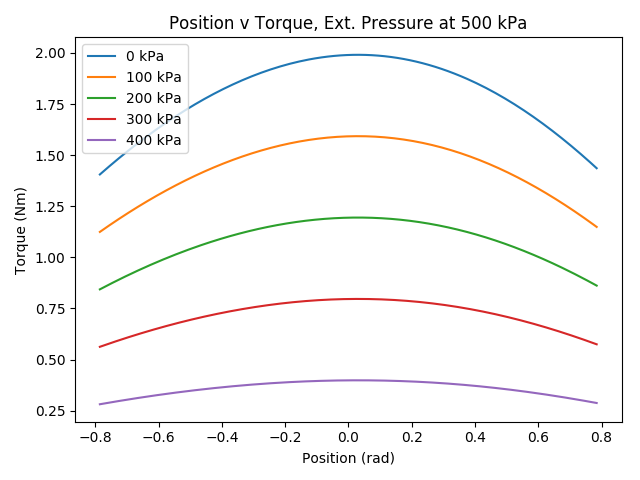
\includegraphics[height=3.5in]{results/Pos_v_AntagTorque}
\caption{Relation between joint position, actuator pressures and
torque applied. Extension actuator pressure was set to 500 kPa and flexion was
set as indicated}
\label{fig:AntagonisticPressureTorque}
\end{figure}

During the characterization of the joint, simulations were run to determine the
dominant effects between intertia, damping and static loads. The relative 
magnitudes of the acceleration, velocity and position are shown in 
\myref{fig:MaxTorque}, along with the
torque. For the simulated joint, the dominant effect was the inertia; however,
for a robot carrying varying loads, this will not always be the case. The 
maximum torque required to execute the known trajectory is also later used as a
metric for measuring the efficiency of the controller. A controller that is too
aggressive for the trajectory (ex. too high gains on a proportional controller)
will request larger than needed torques during trajectory execution. An ideal
controller will always follow the trajectory with the exact torque needed, no 
more, no less, during steady state operation.

\begin{figure}
\centering
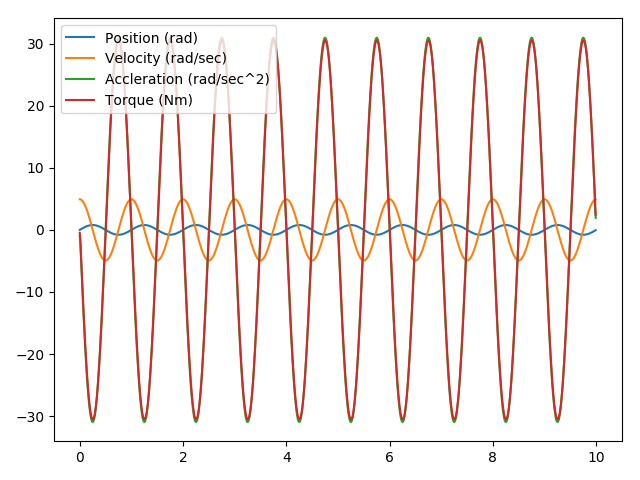
\includegraphics[height=3.5in]{results/Max_Torque}
\caption{Comparing the effects of inertia, damping and static loads. Torque follows acceleration, which suggests that inertia dominates for this simulation}
\label{fig:MaxTorque}
\end{figure}

\section{Python Controller}

The prototype controller written in Python was used to demonstrate the stability
and tracking capabilities of the general algorithm. It was also used to find a
suitable simplification of the internal model that was sufficiently accurate for
optimization but had minimal parameters to tune.

\bbss{Simplified Controller}

The simplified controller demonstrates effective control once the weight updates
were combined with a suitable starting state. \myref{fig:SimplifiedTracking}
demonstrates the progression from original state to a stable and accurate
control of joint position. The blue line is the desired trajectory, with purple
used to highlight error bounds of $\pm$ 1 degree. Orange indicates the actual
position of the joint and the green line indicates the internal state
estimation.

\begin{figure}
\centering
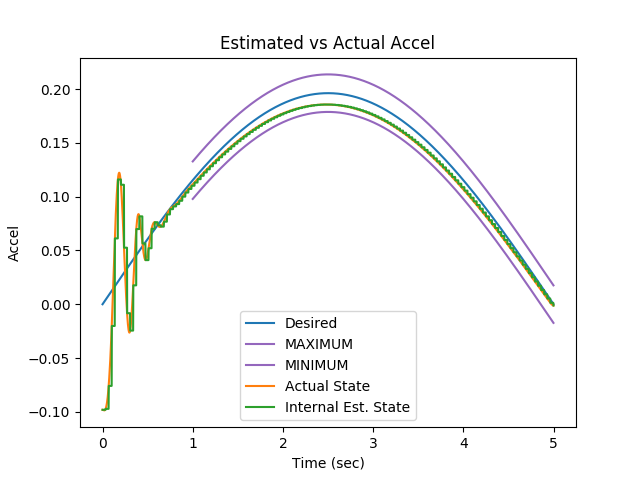
\includegraphics[height=4in]{results/State_Estimation}
\caption{Tracking improves with improved state estimation and internal model
updates}
\label{fig:SimplifiedTracking}
\end{figure}

\bbss{Static Controller}

During testing, the need for an internal model update was verified through 
tests where the optimization loop was applied with variations on correct 
parameters. One example was varying mass. For correct values, such as 
\myref{fig:StateEstimationPerfect}, the system worked within tolerances. When 
mass was underestimated (see \myref{fig:StateEstimationLowMass}), the tracking 
performance degrades to smoothly fail required tracking accuracy. On the other 
hand, over estimating the mass caused aggressive oscillation and underdamping (
see \myref{fig:StateEstimationHighMass}). Based on this data, the assumption 
that the internal model needed to be updated was validated.

\begin{figure}
\centering
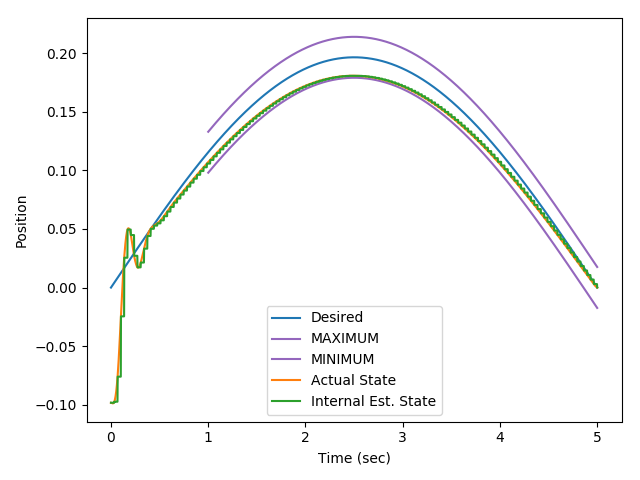
\includegraphics[height=4in]{results/State_Estimation_Perfect}
\caption{Accurate Tracking with a good internal estimation of mass}
\label{fig:StateEstimationPerfect}
\end{figure}

\begin{figure}
\centering
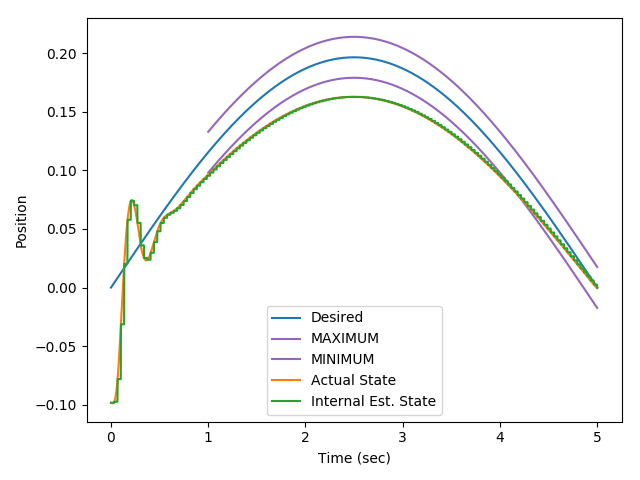
\includegraphics[height=4in]{results/State_Estimation_LowMass}
\caption{Overdamped Tracking with a low internal estimation of mass}
\label{fig:StateEstimationLowMass}
\end{figure}

\begin{figure}
\centering
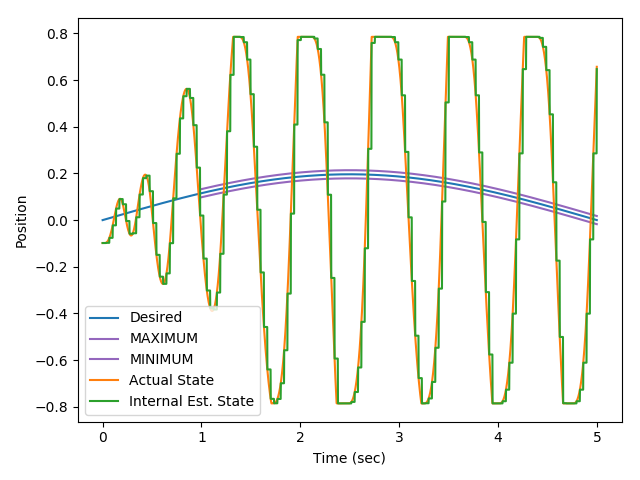
\includegraphics[height=4in]{results/State_Estimation_HighMass}
\caption{Underdamped failure with a high internal estimation of mass}
\label{fig:StateEstimationHighMass}
\end{figure}

\bbss{Simple Parameter Estimation}

The original model for parameter updates was to calculate the sign of the update
and make a uniform incremental change in that direction. In practice, this 
resulted in near-perfect tracking; however, the weight updates themselves were
not intuitive. See \myref{fig:StateUpdateSimple}.

\begin{figure}
\centering
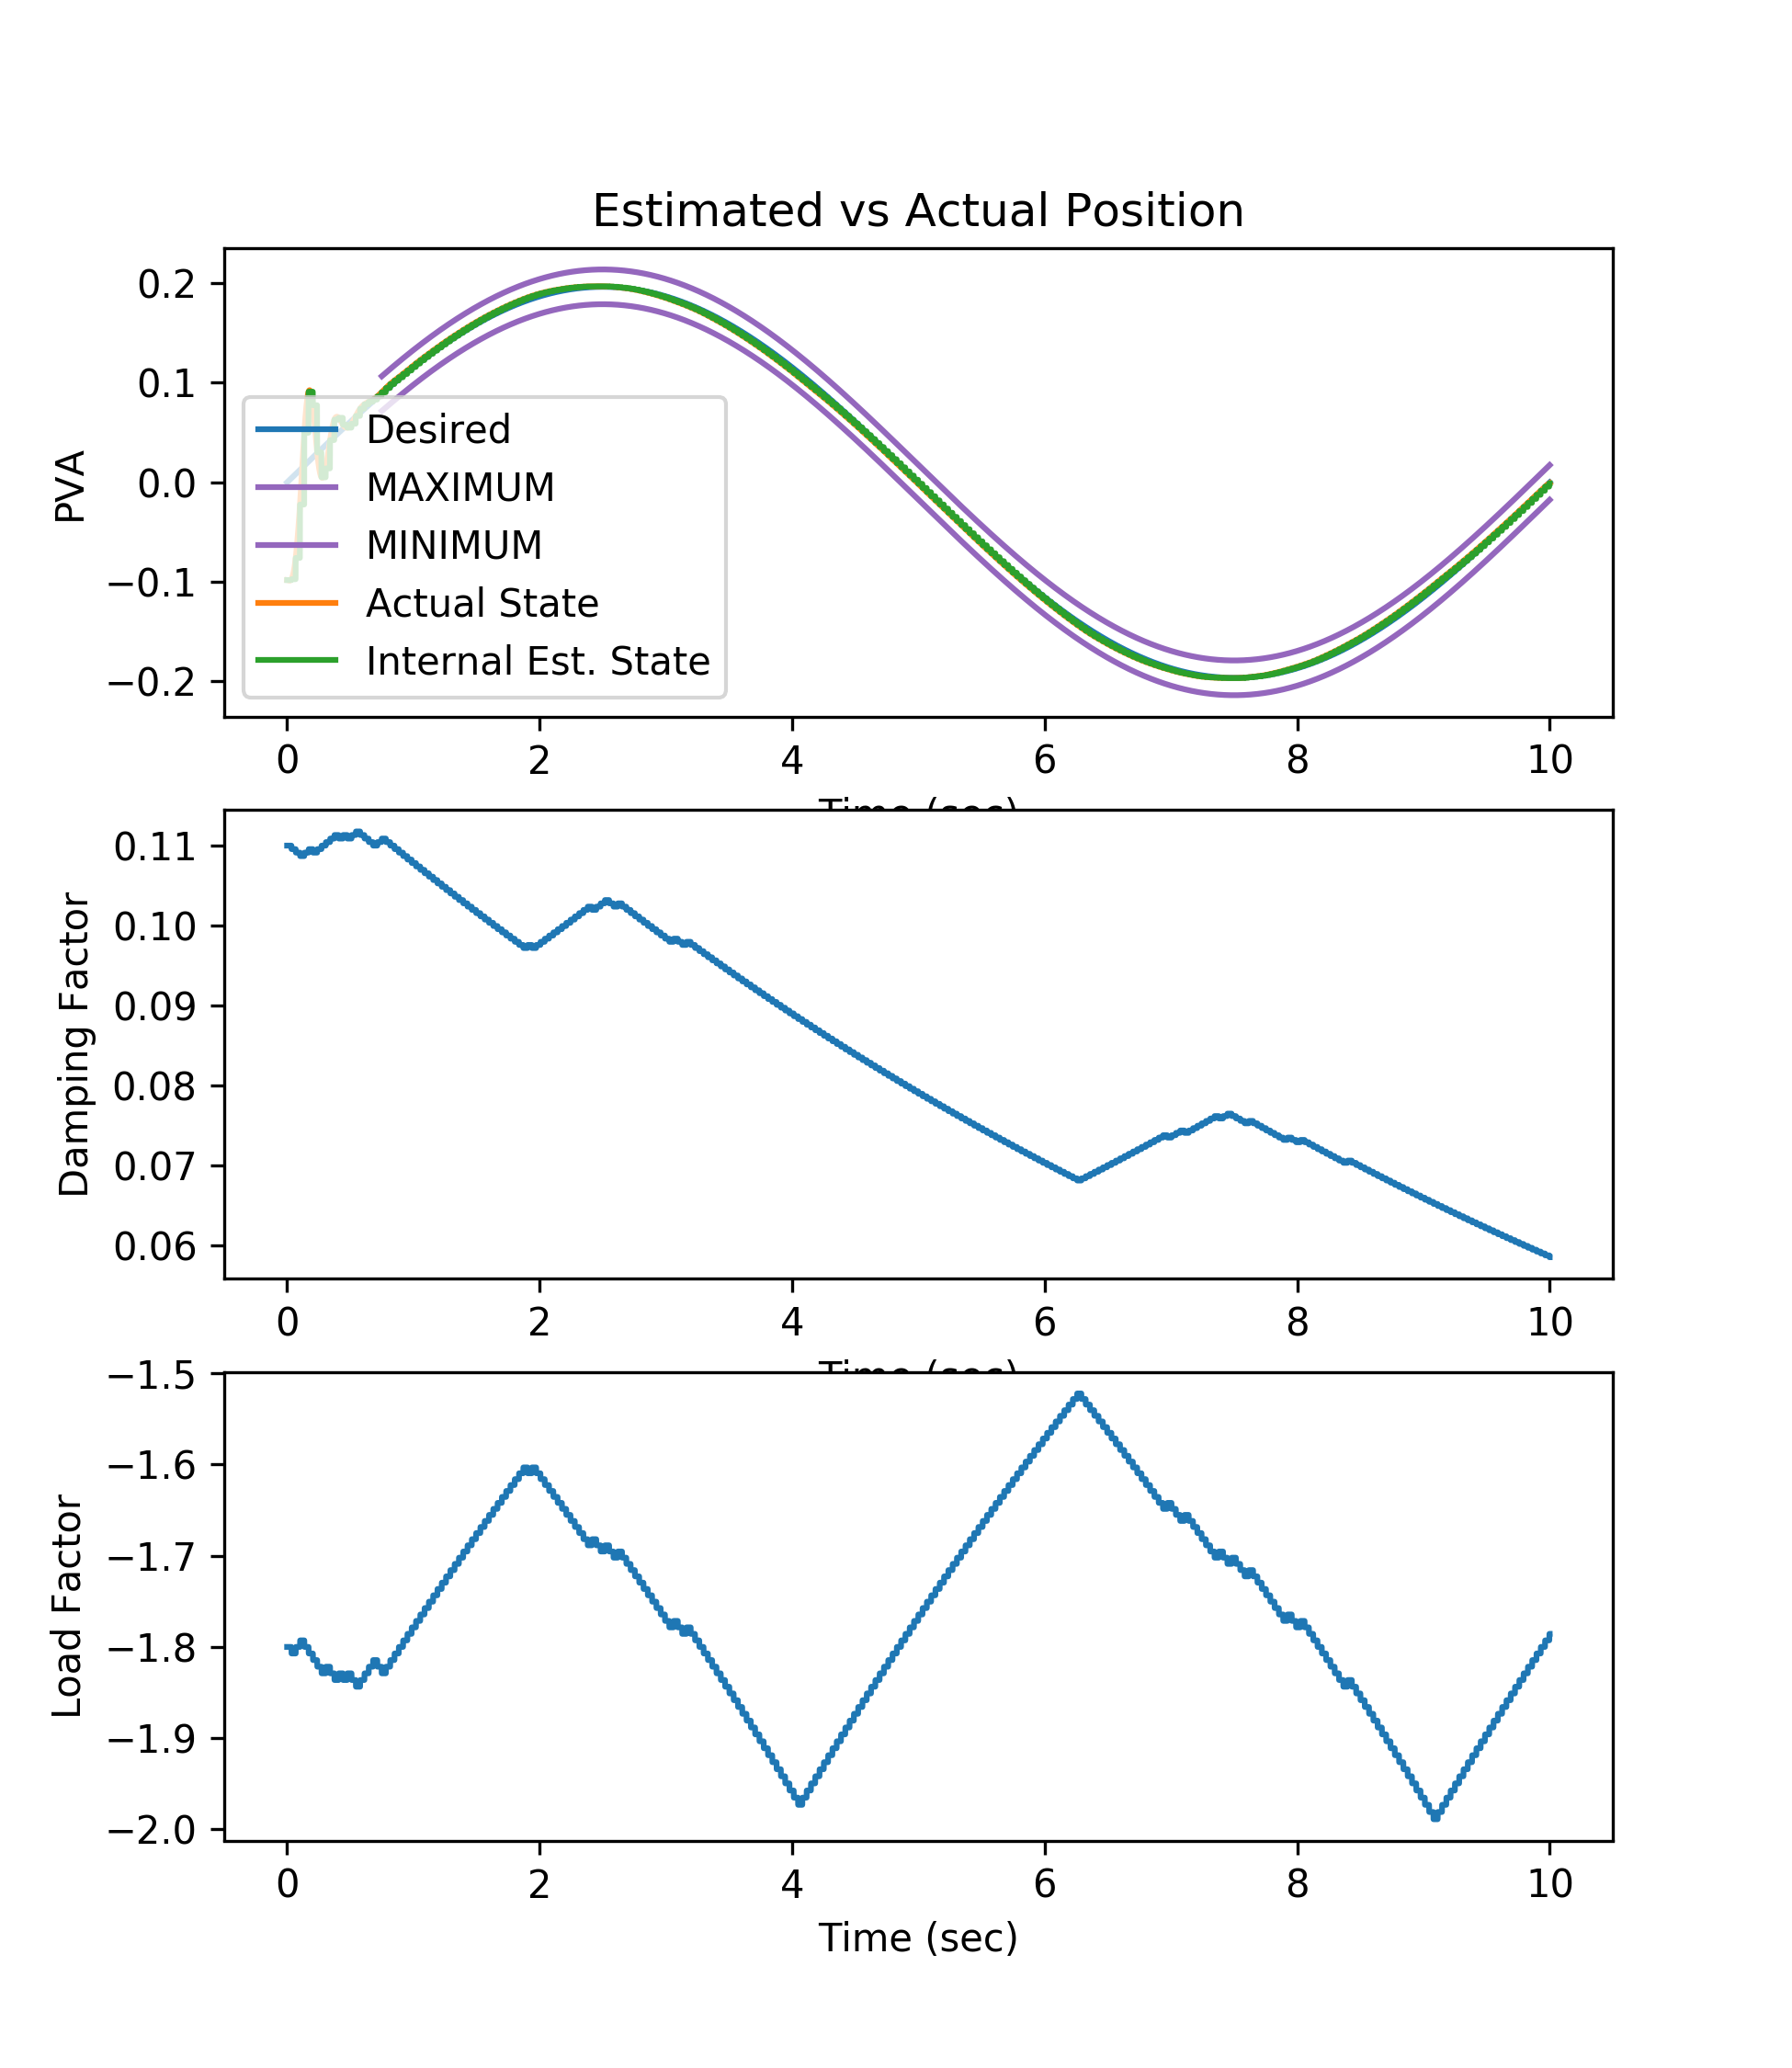
\includegraphics[height=7.5in]{results/State_Model_SimpleUpdate}
\caption{Successful tracking with simple parameter update}
\label{fig:StateUpdateSimple}
\end{figure}

\section{Neuron Controller}

\bbss{Test Results}

\begin{figure}
\centering
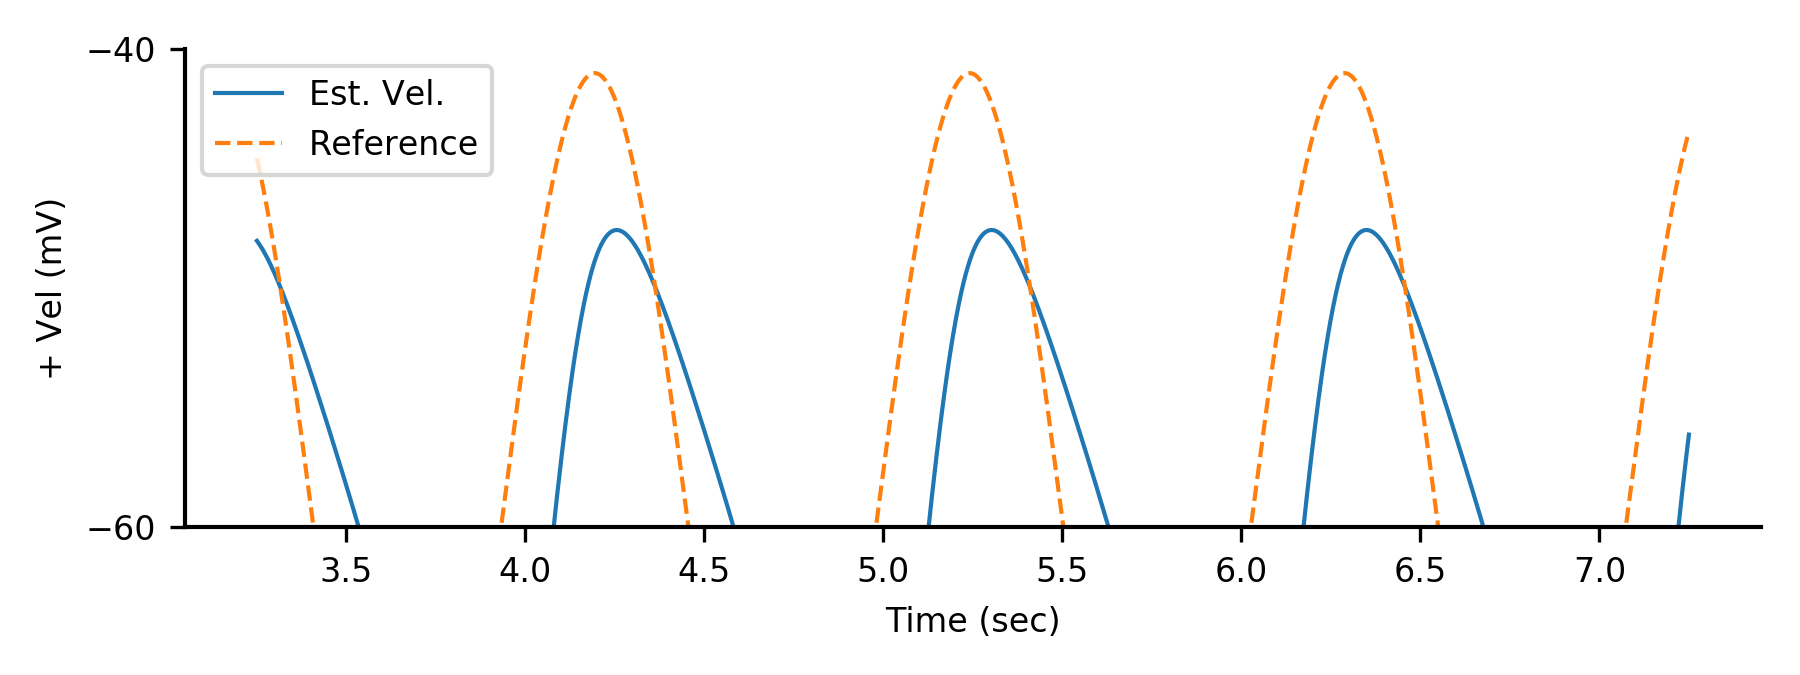
\includegraphics[height=2.25in]{results/TestVelPosWide}
\caption{Testing positive velocity output}
\label{fig:TestVelPos}
\end{figure}

\begin{figure}
\centering
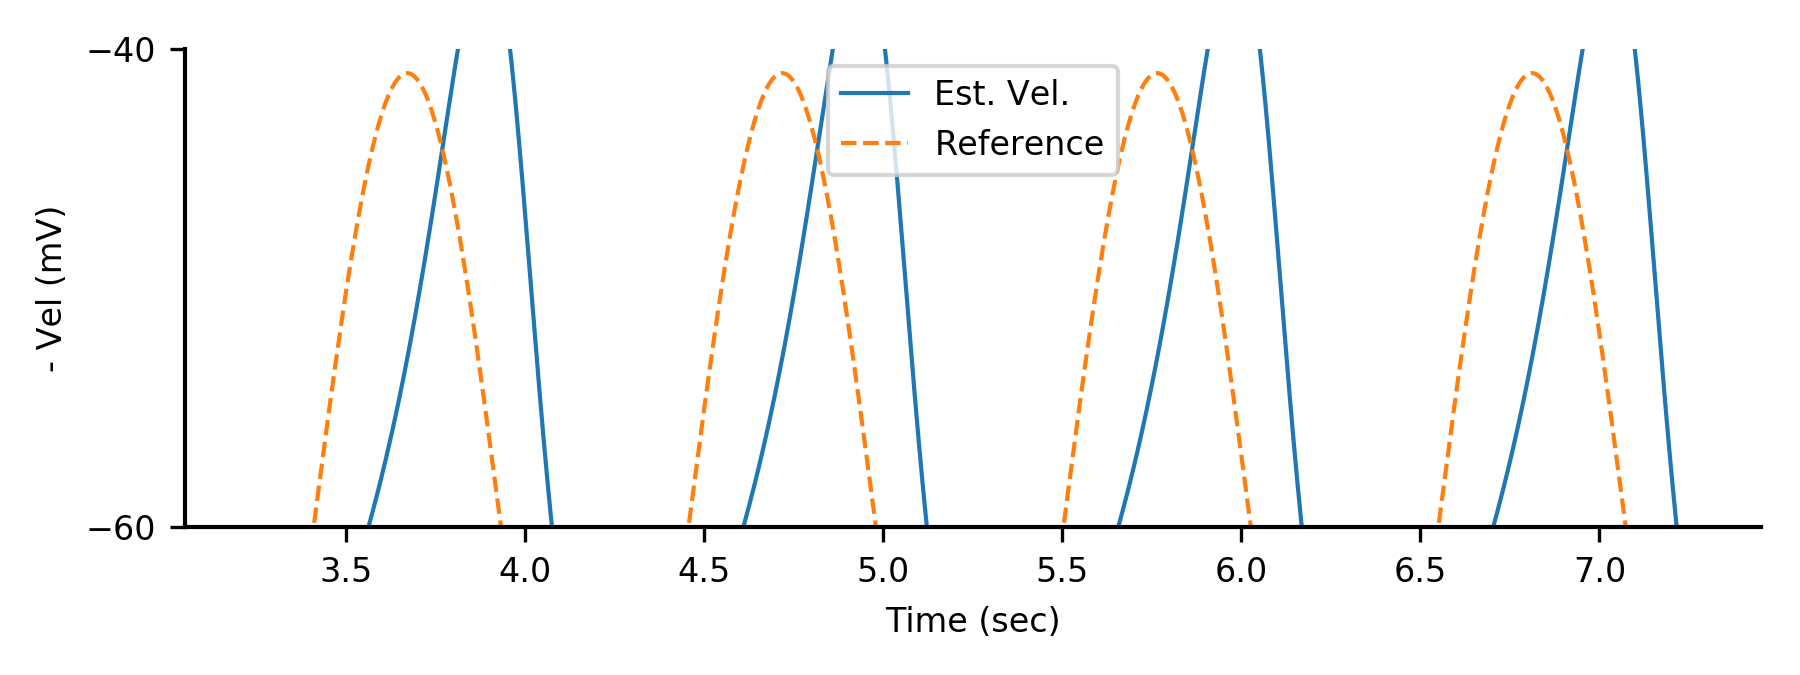
\includegraphics[height=2.25in]{results/TestVelNegWide}
\caption{Testing negative velocity output}
\label{fig:TestVelNeg}
\end{figure}

% TODO(buckbaskin): do something consistent or creative with these captions

\begin{figure}
\centering
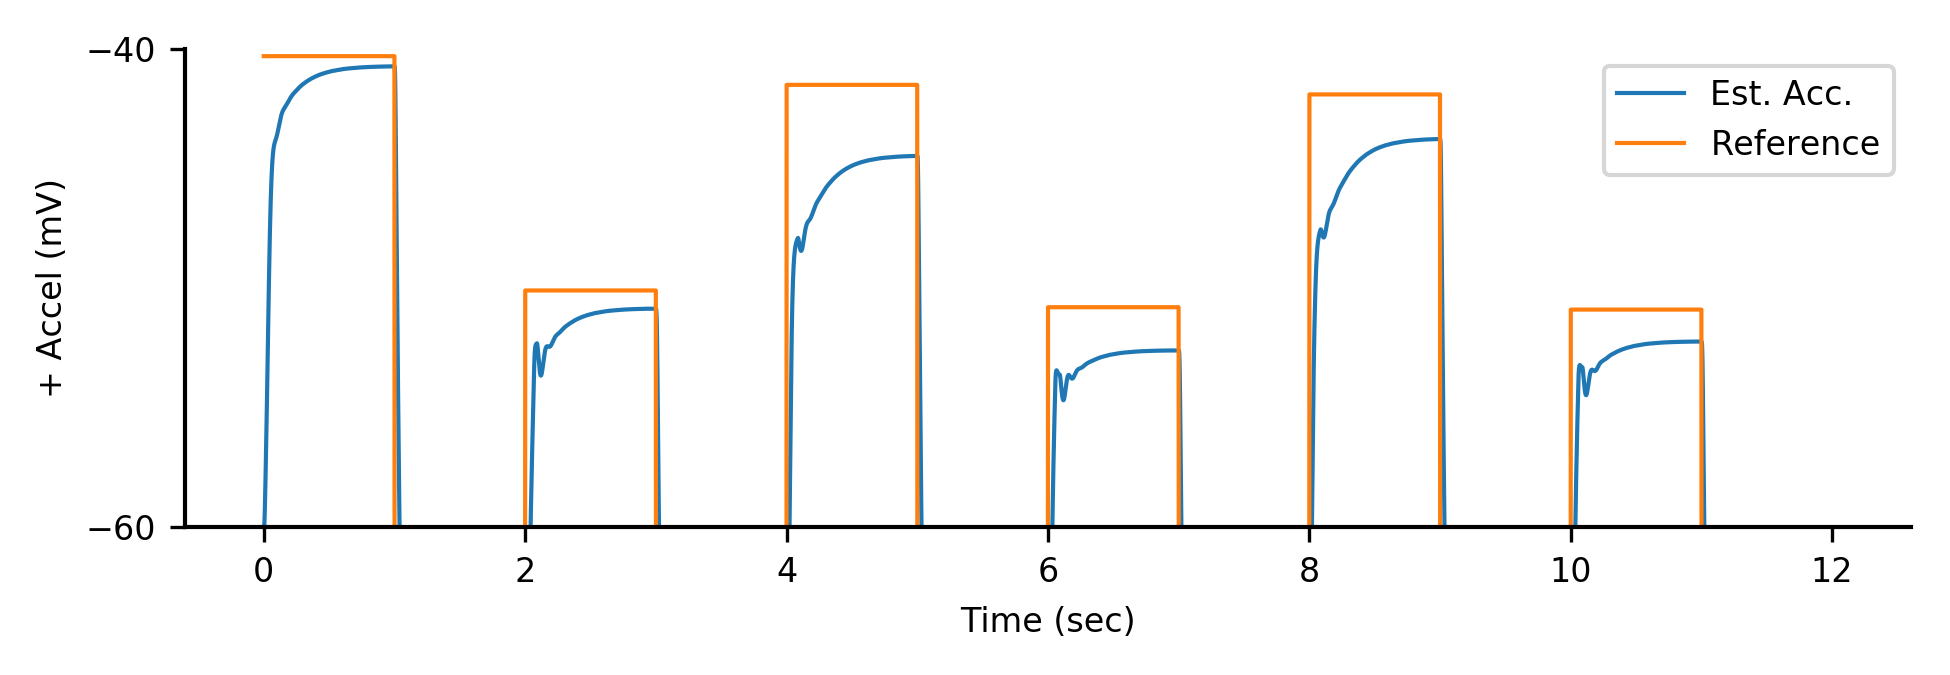
\includegraphics[height=2.25in]{results/TestAccelPosWide}
\caption{Acceleration Testing}
\label{fig:TestAccelPos}
\end{figure}

\begin{figure}
\centering
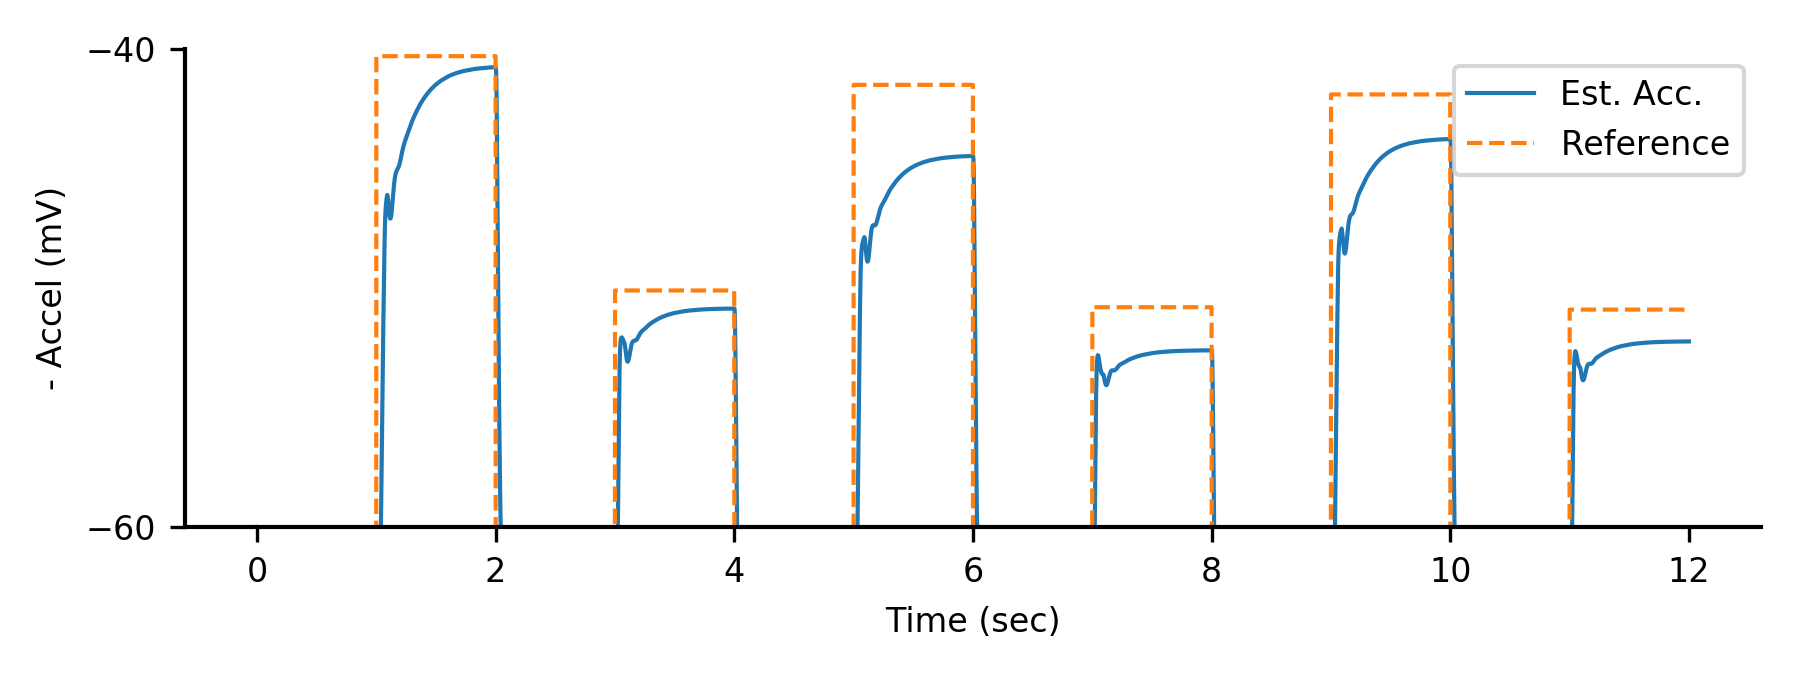
\includegraphics[height=2.25in]{results/TestAccelNegWide}
\caption{Acceleration Testing}
\label{fig:TestAccelNeg}
\end{figure}

\begin{figure}
\centering
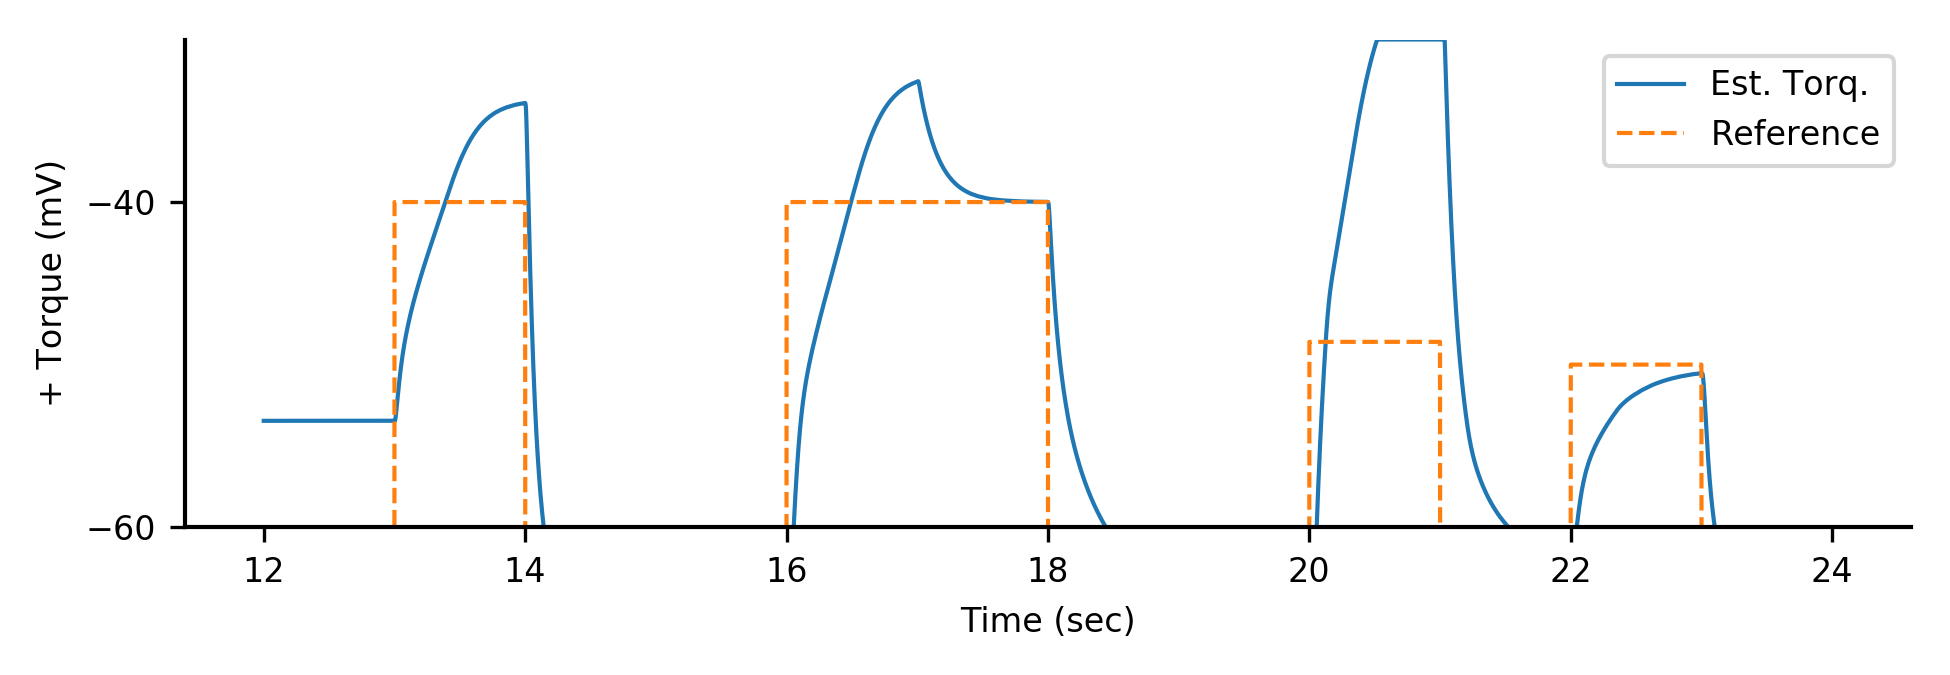
\includegraphics[height=2.25in]{results/TestTorqueOptimizationPosWide}
\caption{Torque Optimization}
\label{fig:TestTorqueOptimizationPos}
\end{figure}

\begin{figure}
\centering
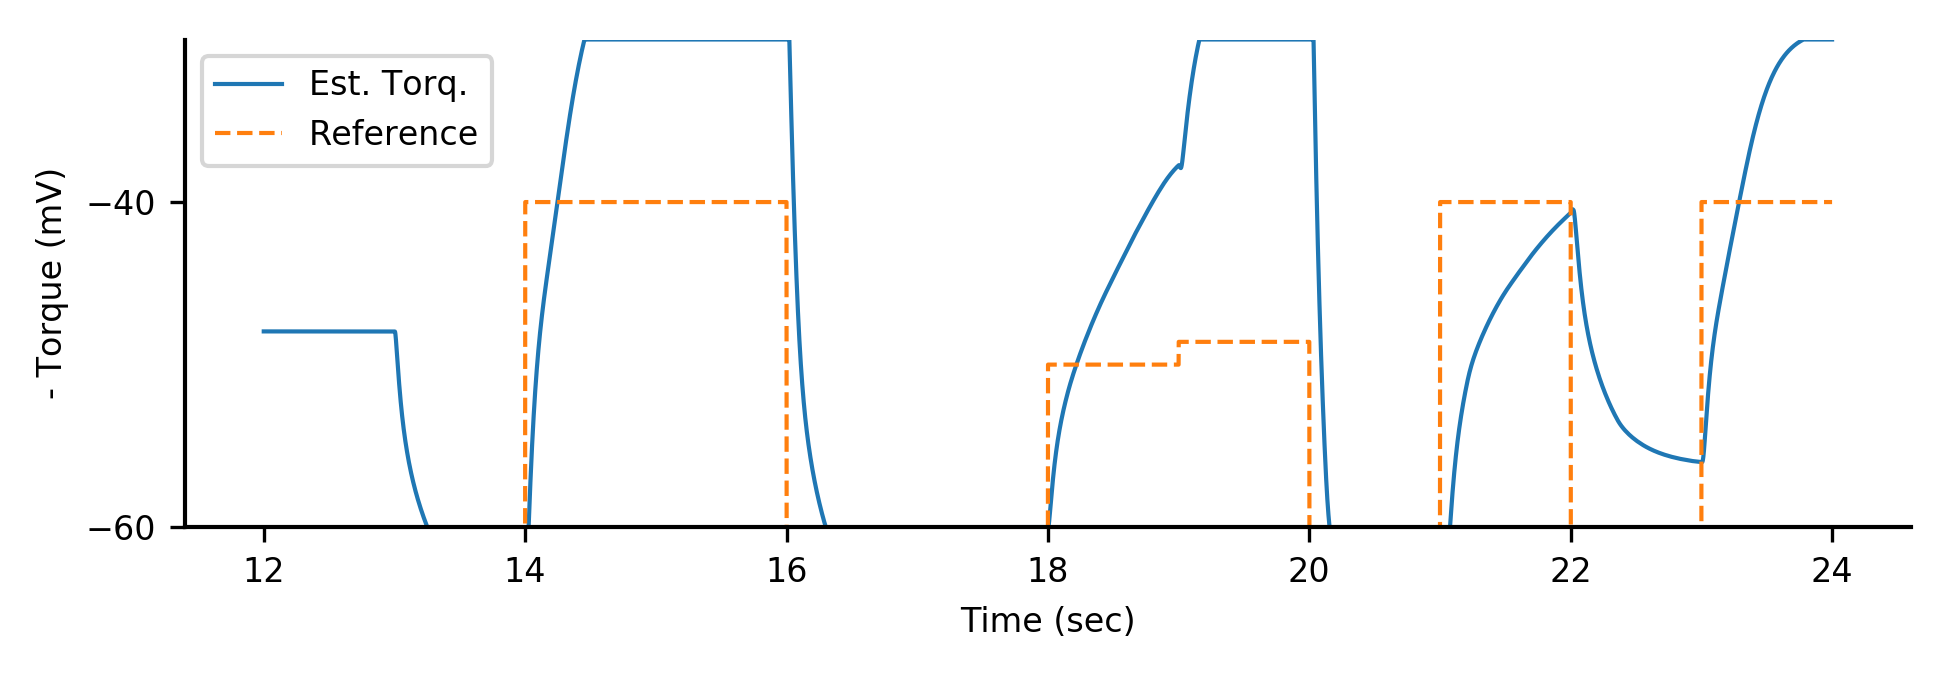
\includegraphics[height=2.25in]{results/TestTorqueOptimizationNegWide}
\caption{Torque Optimization}
\label{fig:TestTorqueOptimizationNeg}
\end{figure}

\begin{figure}
\centering
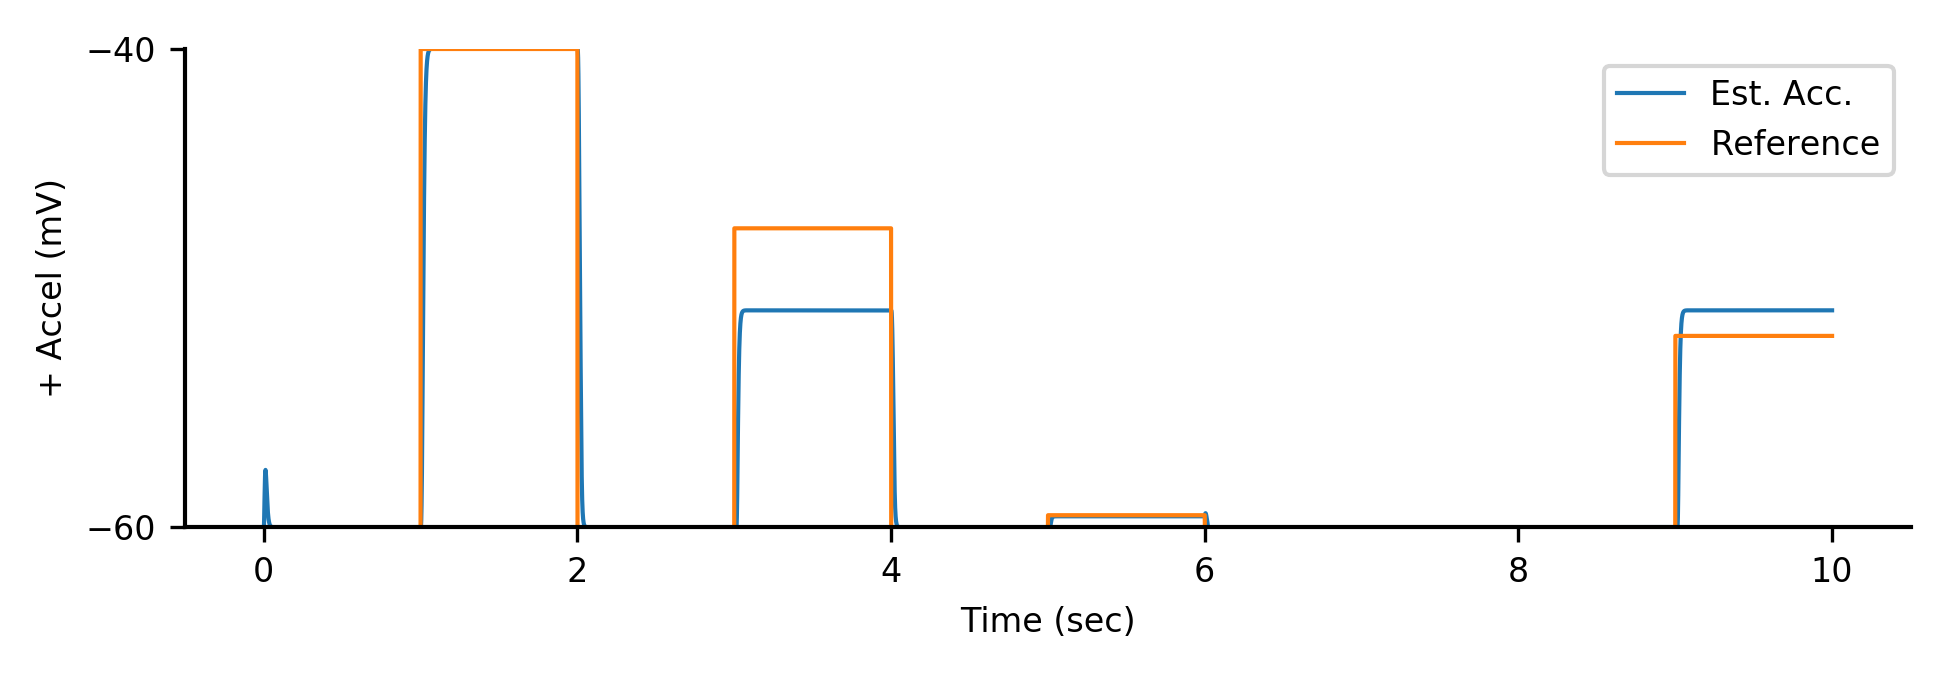
\includegraphics[height=2.25in]{results/TestT2APosWide}
\caption{Estimated Acceleration from Torque}
\label{fig:TestT2APos}
\end{figure}

\begin{figure}
\centering
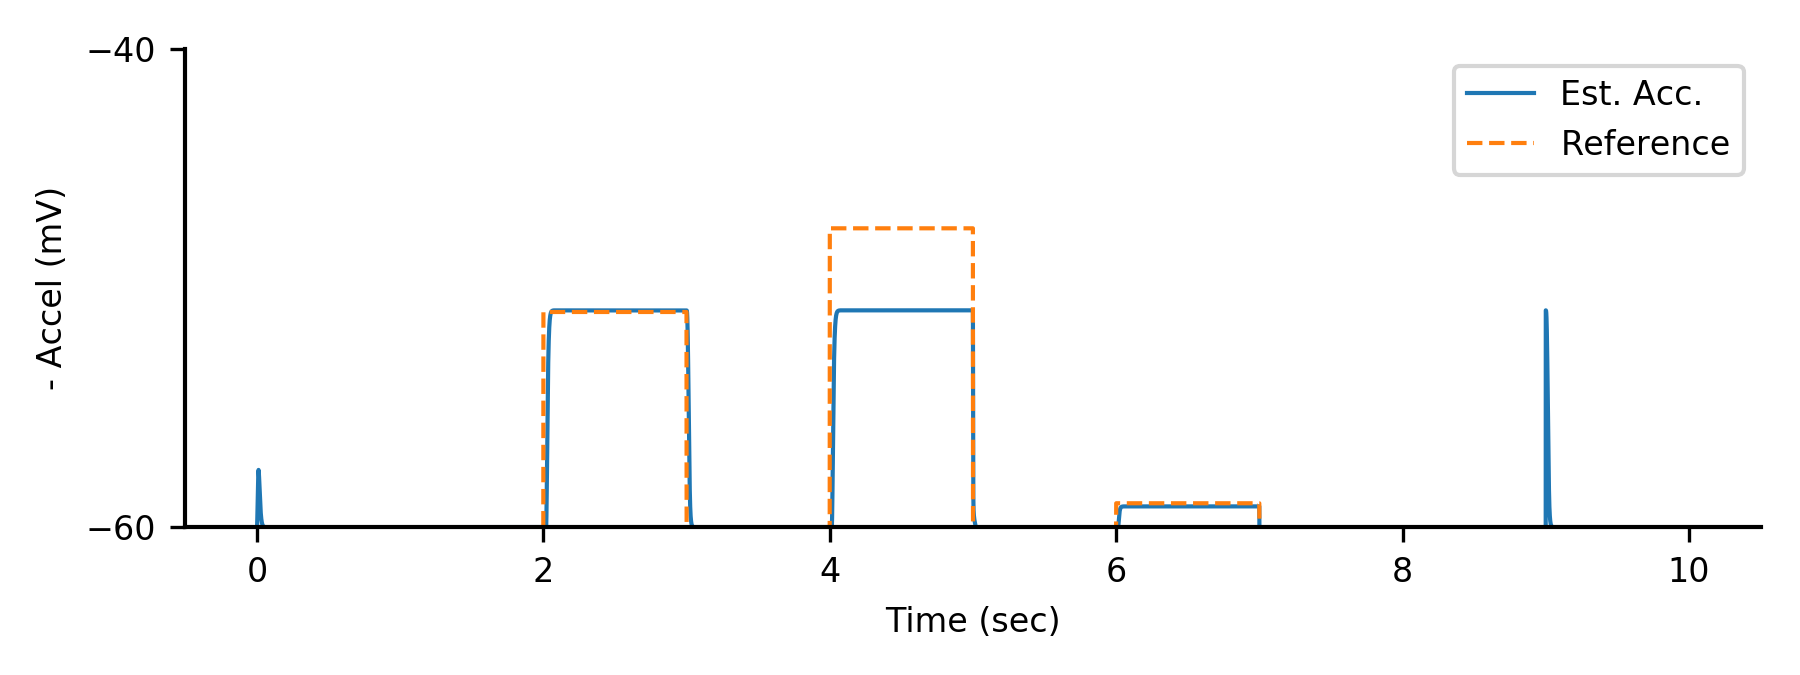
\includegraphics[height=2.25in]{results/TestT2ANegWide}
\caption{Estimated Acceleration from Torque}
\label{fig:TestT2ANeg}
\end{figure}

\begin{figure}
\centering
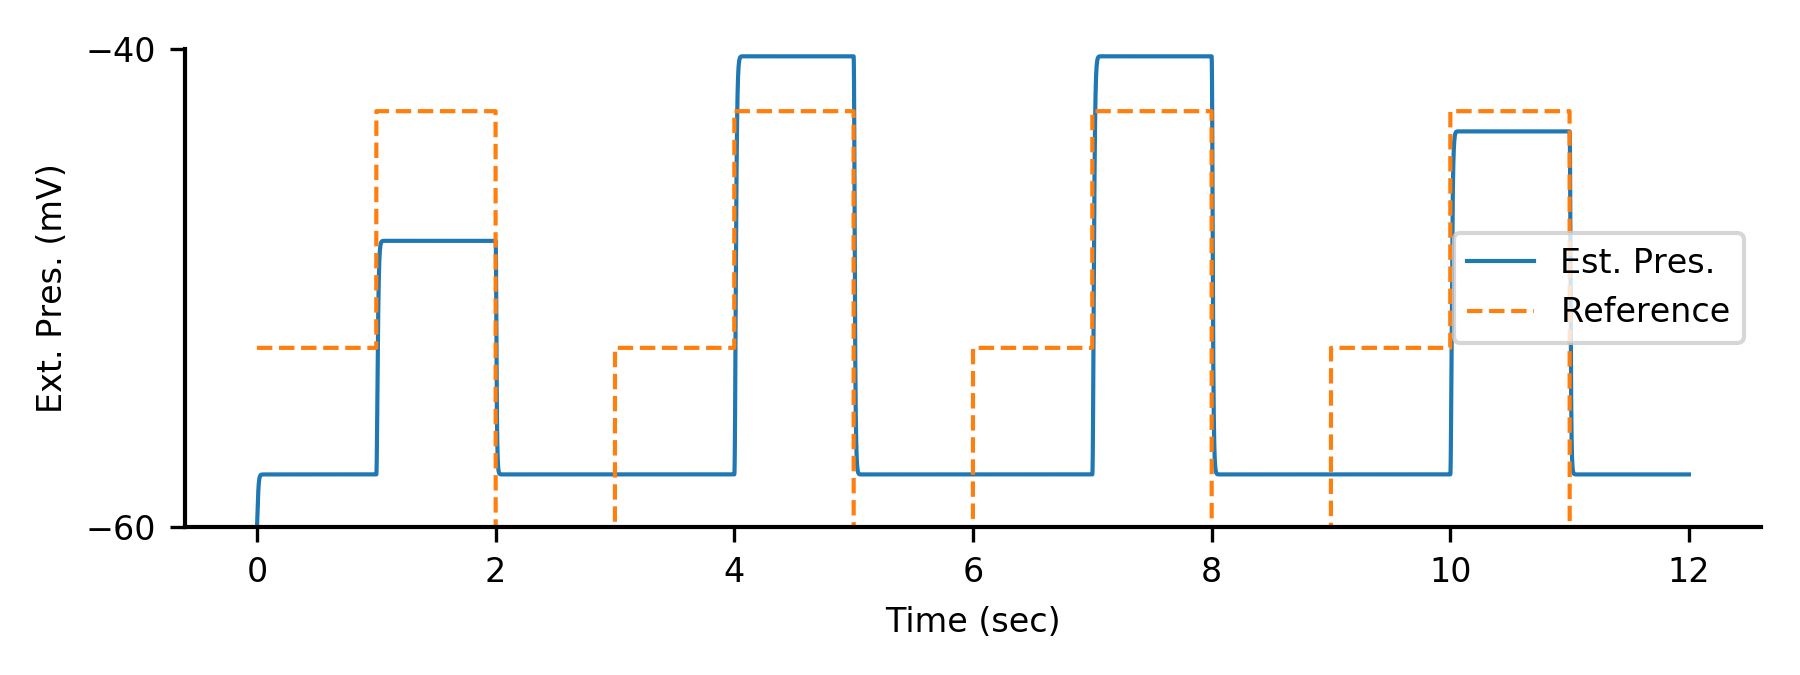
\includegraphics[height=2.25in]{results/TestT2PExtWide}
\caption{Estimated Pressure from Torque}
\label{fig:TestT2PPos}
\end{figure}

\begin{figure}
\centering
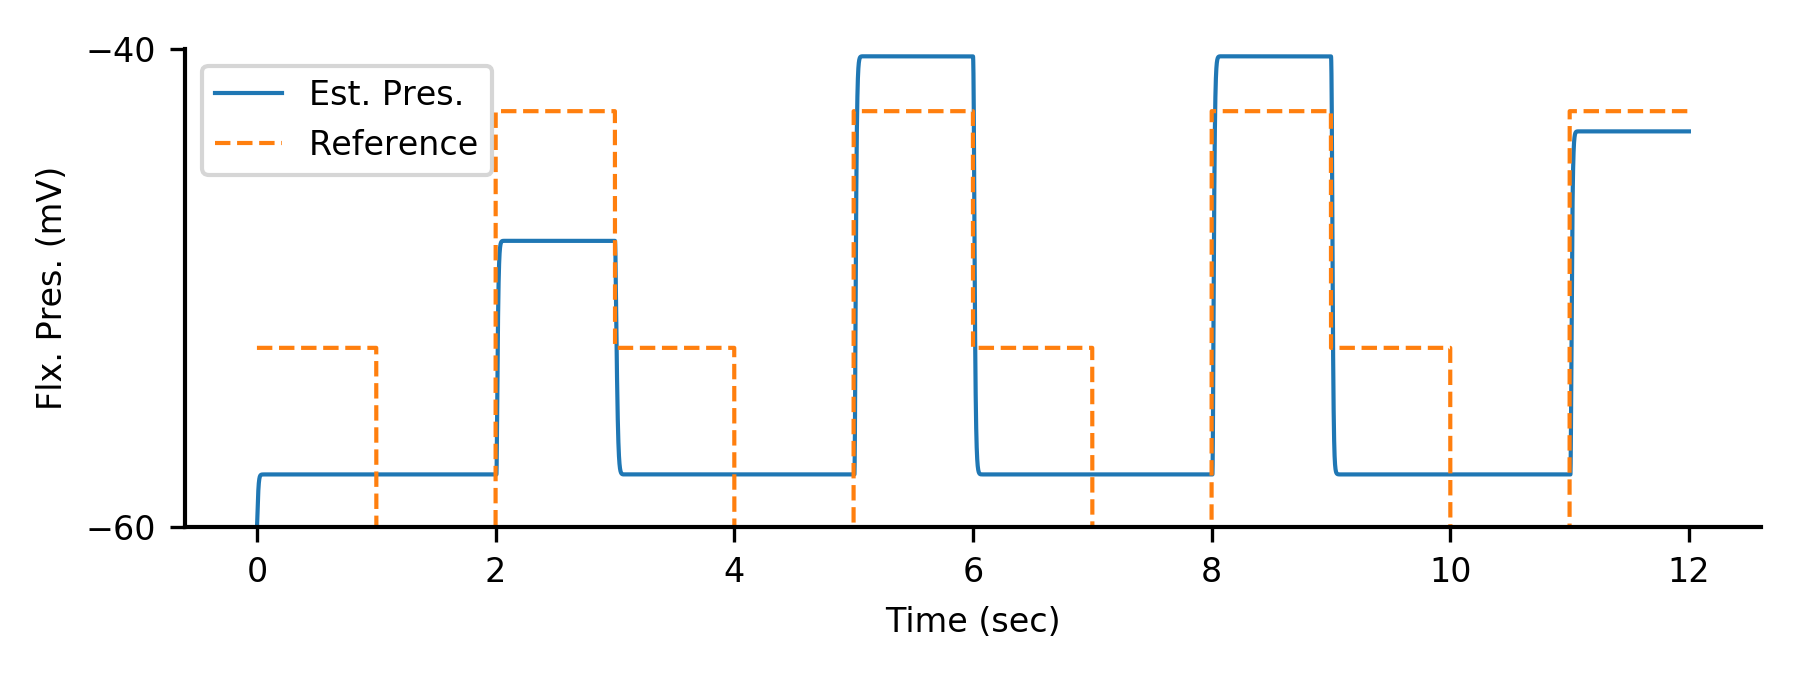
\includegraphics[height=2.25in]{results/TestT2PFlxWide}
\caption{Estimated Pressure from Torque}
\label{fig:TestT2PNeg}
\end{figure}

\begin{figure}
\centering
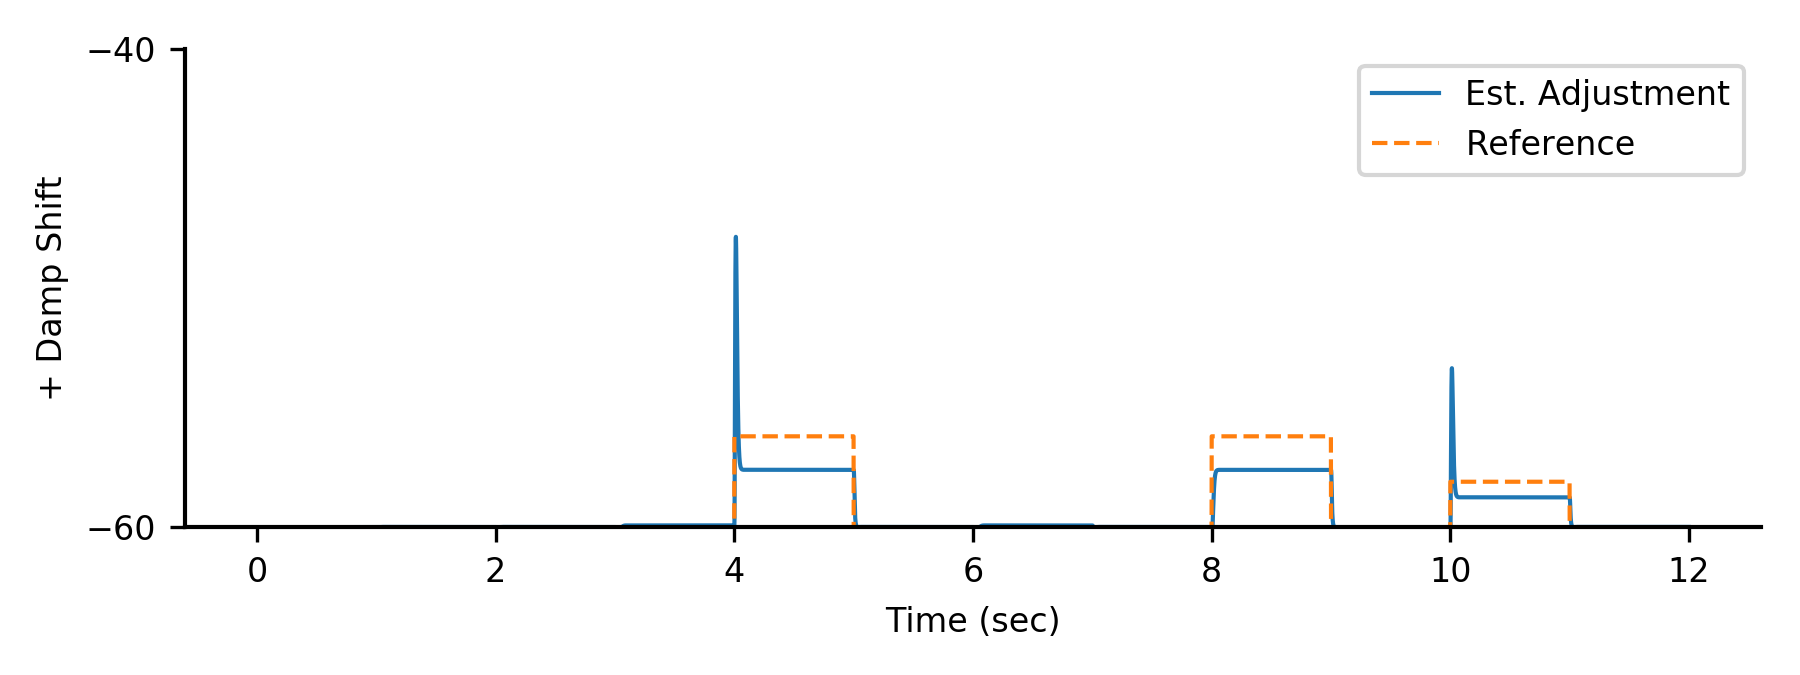
\includegraphics[height=2.25in]{results/TestSystemCPosWide}
\caption{Neuron and actual damping factor updates}
\label{fig:TestSystemCPos}
\end{figure}

\begin{figure}
\centering
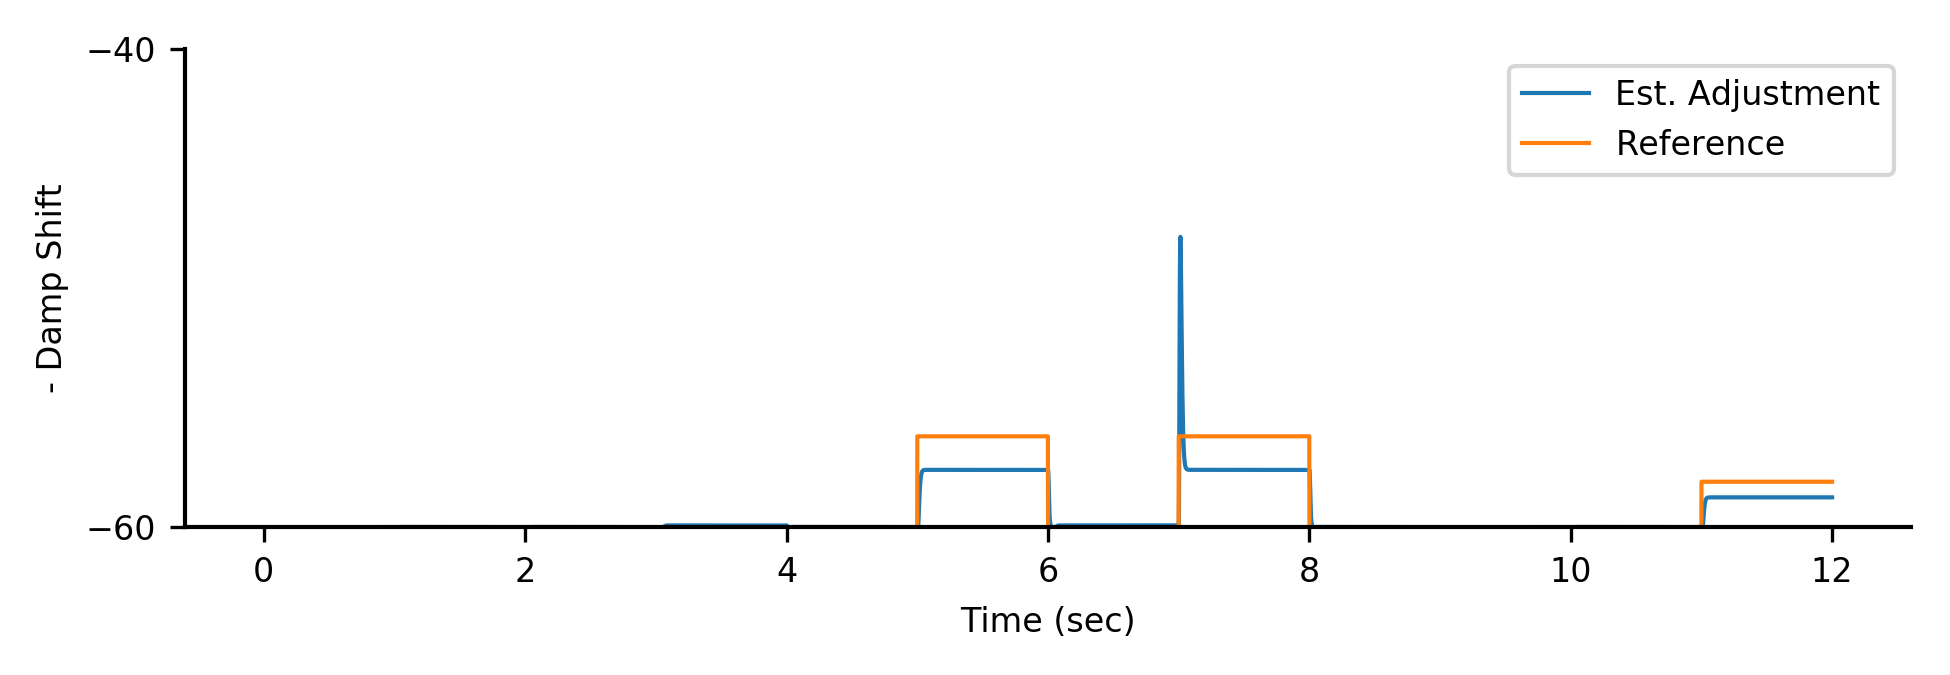
\includegraphics[height=2.25in]{results/TestSystemCNegWide}
\caption{Neuron and actual damping factor updates}
\label{fig:TestSystemCNeg}
\end{figure}

\begin{figure}
\centering
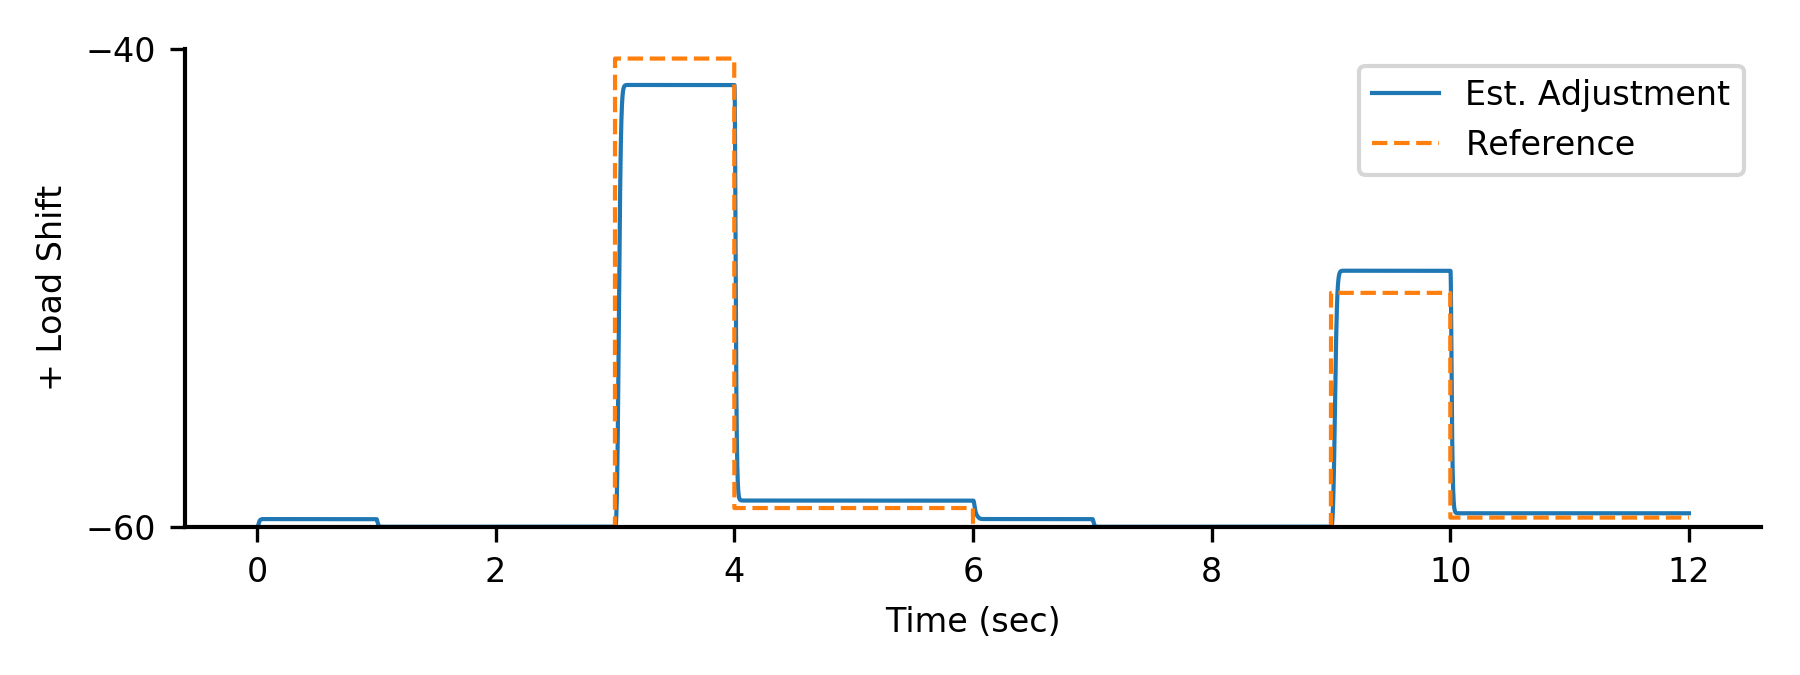
\includegraphics[height=2.25in]{results/TestSystemNPosWide}
\caption{Neuron and actual load factor updates}
\label{fig:TestSystemNPos}
\end{figure}

\begin{figure}
\centering
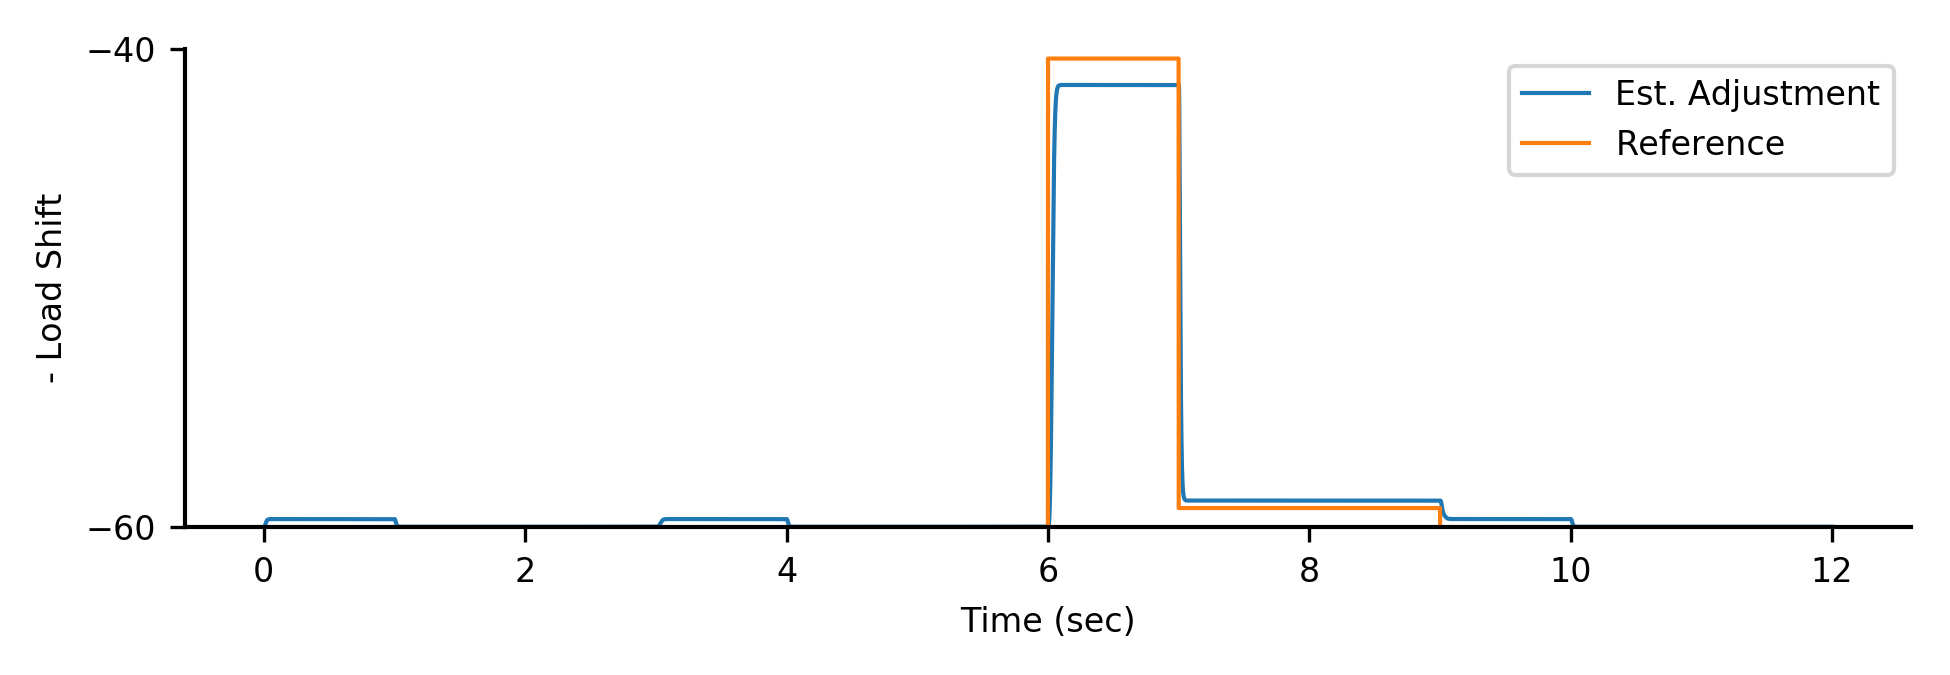
\includegraphics[height=2.25in]{results/TestSystemNNegWide}
\caption{Neuron and actual load factor updates}
\label{fig:TestSystemNNeg}
\end{figure}

\bbsss{Sensor Fusion}

The two key estimates made within the sensor fusion sub-network: velocity and
acceleration. Both controllers were tested against sin waves of known
frequencies. See \myref{fig:TestVelPos} and \myref{fig:TestVelNeg}.
Within the neuron network, acceleration is calculated primarily from actuator
pressures. The output is plotted compared with expected output. See
\myref{fig:TestAccelPos} and \myref{fig:TestAccelNeg}.

\bbsss{Torque Optimization}

The torque optimization network was tested as a complete network. See
\myref{fig:TestTorqueOptimizationPos} and \myref{fig:TestTorqueOptimizationNeg}.
The components for converting the torque to
acceleration were also tested
separately. See \myref{fig:TestT2A}.
The components for converting the torque to pressure were also tested
separately. See \myref{fig:TestT2P}.

\bbss{System Modeling}

The system modeling network was tested as a complete network because both the
damping and load factors are updated from the same $\lambda$ value. See \myref{
fig:TestSystemC} and \myref{fig:TestSystemN}.

\bbss{Discussion}
\label{chap:discussion}

In this paper, we propose a new system for controlling joints actuated with
pneumatic artificial muscles. The design focuses on improving controller
performance through improved sensor processing, an internal optimization step
and an observer that continually updates the internal physics model to improve
the optimization step. This design was implemented as part of a synthetic
nervous system controller, with modifications made to the initial design to aid
in conversion to a neuron and synapse model and to leverage the benefits of the
synthetic nervous system approach.

\bbsss{Sensor Fusion}
\bbssss{Velocity}

The velocity network in the sensor fusion algorithm varies the most from the
reference data. This is a known phenomena addressed in
\cite{NickFunctionalSubnetwork}. This variance is observed in two quantities,
the phase shift and the magnitude

In this particular network, the magnitude of the positive and negative
velocities varied quite widely compared with the reference, especially at
higher gains. During the tuning of the network, a balance was chosen between
the maximum phase lag, minimized by decreasing the time constant of the slower
neuron, and increasing the gain (and therefore the observed difference between
positive and negative velocities).

This error suggests that there is an underlying error in the way that positive
and negative operations are computed; however, through individual tuning the
synapses appear to be relatively accurate. The use of the derivative network
varies in each application across different sub-networks and so the engineering
solution for the correct balance of accuracy, gain and phase varies. This
leaves open the opportunity for biology to inform a single true correct
solution or a more complex derivative network that can independently select for
gain and phase.

\bbssss{Acceleration}

The acceleration network shows effective convergence a near-correct solution.
This demonstrates that the feedback loop concept can be effective; however, it
does take a relatively fixed amount of time to
converge from solutions that are a significant step away. This may lead to
issues with rapidly changing pressures on a hardware system. One potential
solution is to modify the time constants of the network
elements within the loop, in particular the integration network, to allow the
internal loop(s) to run faster than the rest of the network
so they appear to converge to the correct value on the same time scale as the
rest of the network.

\bbsss{Torque Optimization}

The torque optimization network shows that in many cases it converges to the
correct solution; however, like the feedback in the acceleration network, it can
take a long time to converge to the correct solution from discontinuous starting
values. Due to the integrator included in the network, the starting conditions
for the first test case are based on other tests and didn't show consistent
behavior.

The concept of the torque optimization network appears to be effective; however,
its implementation in neurons suffers from both attempting to converge to a
solution quickly and approximating a physical simulation internally. The network
uses relatively low time constants and high gains. This can cause overshoot
(not seen in \myref{fig:TestTorqueOptimization} due to clipping) where the
estimated torque is off the charts for either large positive or negative swings.
The high gains also reduce accuracy by amplifying small errors made during the
approximation of the ``physics" implementation. This behavior replicates
observations made during the development of the prototype controller in code,
where an attempt to approximate the physics of the joint in a single step was
inaccurate. The solution to this was to make multiple iterations by subdividing
the simulated time so that a simpler physics model would have a closer fit to
the actual dynamics. This suggests that a longer string of neurons would be
necessary within the loop to project dynamics forward; however, this may
increase timing issues with the network when interfaced to hardware.

\bbssss{Acceleration from Torque}

The 3 stage network for estimating the acceleration from the torque applied to
the system appears to work well. There are two test cases, between 7 and 9
seconds that were not significant when tested at the resolution that the
network incorporates. Otherwise, the acceleration is almost always correct.
Given its intended uses, the network is sufficiently accurate and suggests that
relatively small sets of neurons can provide a representation of the physics of
a biological system. This would suggest that an animal's nervous system can
relatively easily understand the dynamics of its environment and its body.

\bbssss{Estimating Pressures from Torques}

The process for calculating pressures from torques is accurate in some
cases and inaccurate in many others. This suggests that the physical
model of the pneumatic artificial muscles proposed in \cite{HuntPMuscles}
doesn't convert well to a relatively small network of neurons. This would
suggest that a future controller iteration might move the mechanical
calculation of this conversion out of neurons and
to LabView other other code used to interface between synthetic neurons and
hardware.

\bbsss{System Model}

The network for predicting the weight update is very accurate and suggests that
the engineered process of estimating the modeling errors of a synthetic neuron
network within the network itself is both feasible and an effective process for
the continual improvement of a controller applied to a particular hardware
joint under control.

This application is also generally more suitable to neuron networks than say,
the calculation of the conversion from pressures to torques following a well
prescribed algorithm involving a shifted tangent function. The exact magnitude
of the update of the weights, especially at a reduced gain, is not as important
as the relative magnitude and sign of each update. This means that the
implementation of an arithmetic operation or dynamic calculation by a synapse of
a collection of synapses is tolerant to small variances from the expected
behavior.
